% Drawing 154/07-16 -- folder 154, batch 07, archive page 139 (PDF page 140).
% Transcription: dessins au crayon et à l'encre brune : une sphère coupée par un équateur en tirets, les points $-1$, $+1$, $0$, $\infty$ et un méridien épais ; au-dessous, une sphère au crayon traversée de méridiens, le point $0$ en haut, avec une légende illisible ; au milieu, un ovale brun (moitié en tirets) aux points $0$, $\infty$, $-1$, $+1$ ; en haut à droite, deux dômes au crayon aux méridiens marqués, avec les points $-1$, $0$, $+1$
% Kind: spheres with equator, points -1, +1, 0, infinity and meridians. Method 2 (schematic redraw from the facsimile). Status: partial.
% Notes: Pencil and brown ink drawings, read from the page view: a sphere cut by a dashed equator, the points -1, +1, 0, infinity and a thick meridian; below, a pencil sphere crossed by meridians, the point 0 at the top, with an illegible legend (left out); in the middle, a sphere seen from the side, points 0 (top), infinity (bottom), -1, +1 and a dashed meridian; top right, two pencil domes with marked points (-1, +1, 0) drawn in outline. Still differs from the facsimile: Pencil and brown ink drawings, read from the page view: a sphere cut by a dashed equator, the points -1, +1, 0, infinity and a thick meridian; below, a pencil sphere crossed by meridians, the point 0 at the top, with an illegible legend (left out); in the middle, a sphere seen from the side, points 0 (top), infinity (bottom), -1, +1 and a dashed meridian; top right, two pencil domes with marked points (-1, +1, 0) drawn in outline.
% Coordinates: 1 unit = 1 mm = 1/100 of the crop width (bbox in page fractions: [0.157, 0.124, 0.927, 0.502]).
% Redrawn by Claude (claude-opus-5-5), issue #73, 2026-11-07; not checked by a human; not compiled (no TeX in the session).
% Revised by Claude (claude-opus-5-5) 2026-11-09 (issue #128) after Michel's check: vertices snapped to exact intersections (drawn points on their lines, meeting ends on the stroke they meet, near-concurrent lines through one computed point, curve ends on their rim); labels at \small as in folder 80 batch 3. Status: partial.
% Rights: reproduces part of the work -- behind RENDER_TRANSCRIPTS, never published by itself.
\documentclass[tikz,border=3pt]{standalone}
\usepackage{amsmath,amssymb}
\usetikzlibrary{patterns,arrows.meta}
\tikzset{Or/.style={orange!90!black}, Ye/.style={yellow!80!orange}, Lg/.style={green!60!black!70}, Dg/.style={green!45!black}, Br/.style={brown!80!black}, Rd/.style={red!85!black}, Bl/.style={blue!70!black}, Gy/.style={black!40}, pencil/.style={black!45}, struck/.style={black!35}, mark/.style={circle,draw,inner sep=1.3pt}, pt/.style={circle,fill,inner sep=0.9pt}, opt/.style={circle,draw,fill=white,inner sep=1.1pt}}
\begin{document}
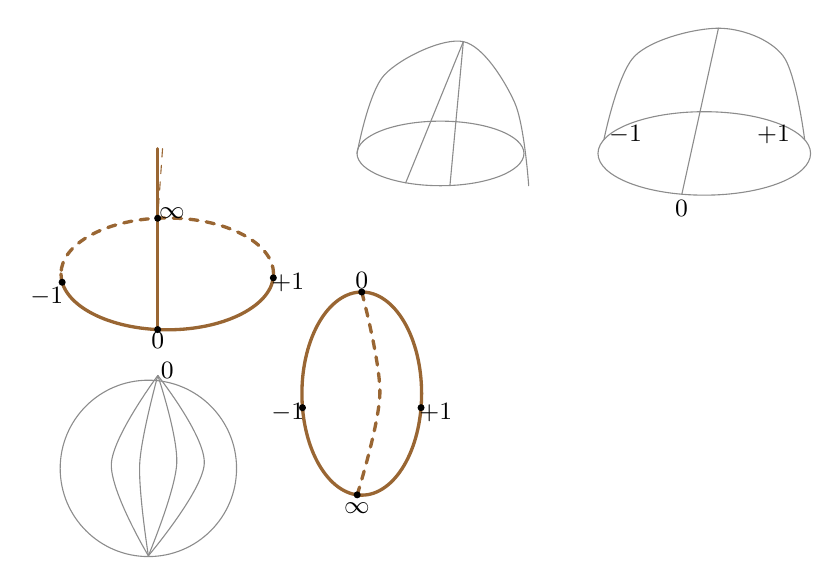
\begin{tikzpicture}[x=1mm,y=1mm,line cap=round,line join=round,font=\scriptsize]
\draw[Br,very thick] (2.4,-32.4) arc[start angle=180, end angle=360, x radius=13.5, y radius=7.1];
\draw[Br,dashed,very thick] (29.4,-32.4) arc[start angle=0, end angle=180, x radius=13.5, y radius=7.1];
\draw[Br,very thick] (14.68,-16.5) -- (14.68,-39.47);
\draw[Br,dashed] (15.3,-16.5) -- (14.68,-25.33);
\node[pt] at (2.55,-33.46) {};
\node[pt] at (29.37,-32.9) {};
\node[pt] at (14.68,-39.47) {};
\node[pt] at (14.68,-25.33) {};
\node[inner sep=1pt] at (0.6,-35.3) {\small $-1$};
\node[inner sep=1pt] at (31.2,-33.5) {\small $+1$};
\node[inner sep=1pt] at (14.7,-40.9) {\small $0$};
\node[inner sep=1pt] at (16.5,-24.7) {\small $\infty$};
\draw[pencil] (13.5,-57.1) circle[radius=11.2];
\draw[pencil] plot[smooth, tension=0.55] coordinates {(14.7,-45.3) (8.8,-56.5) (13.5,-68.2)};
\draw[pencil] plot[smooth, tension=0.55] coordinates {(14.7,-45.3) (12.4,-56.5) (13.5,-68.2)};
\draw[pencil] plot[smooth, tension=0.55] coordinates {(14.7,-45.3) (17.1,-56.5) (13.5,-68.2)};
\draw[pencil] plot[smooth, tension=0.55] coordinates {(14.7,-45.3) (20.6,-56.5) (13.5,-68.2)};
\node[inner sep=1pt] at (15.9,-44.7) {\small $0$};
\draw[Br,very thick] (40.6,-47.6) ellipse[x radius=7.6, y radius=12.9];
\draw[Br,dashed,very thick] plot[smooth, tension=0.55] coordinates {(40.6,-34.7) (42.9,-47.6) (40.02,-60.46)};
\node[pt] at (40.6,-34.7) {};
\node[pt] at (40.02,-60.46) {};
\node[pt] at (33.07,-49.39) {};
\node[pt] at (48.13,-49.39) {};
\node[inner sep=1pt] at (40.6,-33.2) {\small $0$};
\node[inner sep=1pt] at (40,-62.1) {\small $\infty$};
\node[inner sep=1pt] at (31.2,-50) {\small $-1$};
\node[inner sep=1pt] at (50,-50) {\small $+1$};
\draw[pencil] plot[smooth, tension=0.55] coordinates {(40,-17.1) (43.5,-7.1) (53.5,-2.9) (60,-10.6) (61.8,-21.2)};
\draw[pencil] (50.6,-17.1) ellipse[x radius=10.6, y radius=4.1];
\draw[pencil] (53.5,-2.9) -- (51.8,-21.17);
\draw[pencil] (53.5,-2.9) -- (46.18,-20.83);
\draw[pencil] plot[smooth, tension=0.55] coordinates {(71.35,-15.36) (75.3,-4.7) (85.9,-1.2) (94.1,-4.7) (96.85,-15.36)};
\draw[pencil] (84.1,-17.1) ellipse[x radius=13.5, y radius=5.3];
\draw[pencil] (85.9,-1.2) -- (81.25,-22.28);
\node[inner sep=1pt] at (74.1,-14.7) {\small $-1$};
\node[inner sep=1pt] at (92.9,-14.7) {\small $+1$};
\node[inner sep=1pt] at (81.2,-24.1) {\small $0$};
\end{tikzpicture}
\end{document}
